\documentclass{beamer}


% Encoding
    \usepackage[utf8]{inputenc} % für input utf8
    \usepackage[T1]{fontenc}    % Schriftcodierung mit UTF-8
    \usepackage{textcomp}       % Erweiterung von fontenc
    \usepackage{lmodern}        % Erweiterung des Zeichensatzes

% Anpassungen für die Deutsche
    \usepackage[ngerman]{babel} % Neue deutsche Rechtschreibung
    
    % Source-Code Paket
    \usepackage{listings}



\usepackage{todo}
\usepackage{beamerthemeshadow}
\beamersetuncovermixins{\opaqueness<1>{25}}{\opaqueness<2->{15}}
\begin{document}


\title{Recap: Queue, Semaphore, Mutex}  
\author{Silvio Emmenegger\, Pascal H\"afliger}
\date{\today} 

\begin{frame}
\titlepage
\end{frame} 


\begin{frame}
\frametitle{Inhaltsverzeichnis}
\tableofcontents[
  currentsection,
  sectionstyle=show,
  subsectionstyle=hide
]
\end{frame} 

% Pixhawk
\begin{frame}
  \begin{center}
    FRTOS:\\
    H\"ohere Priorit\"at = Wichtiger\\
    %\bigskip 
    %ARM:\\
    %Tiefere Priorit\"at = Wichtiger
  \end{center}
\end{frame}


\section{Queue}
\begin{frame}
	%\frametitle{Queue}
  \tableofcontents[
	    currentsection, 
	    hideothersections, 
	    sectionstyle=show/shaded, 
	    subsectionstyle=hide
	]
\end{frame}


\begin{frame}
  \frametitle{Queue}

  \begin{figure}
  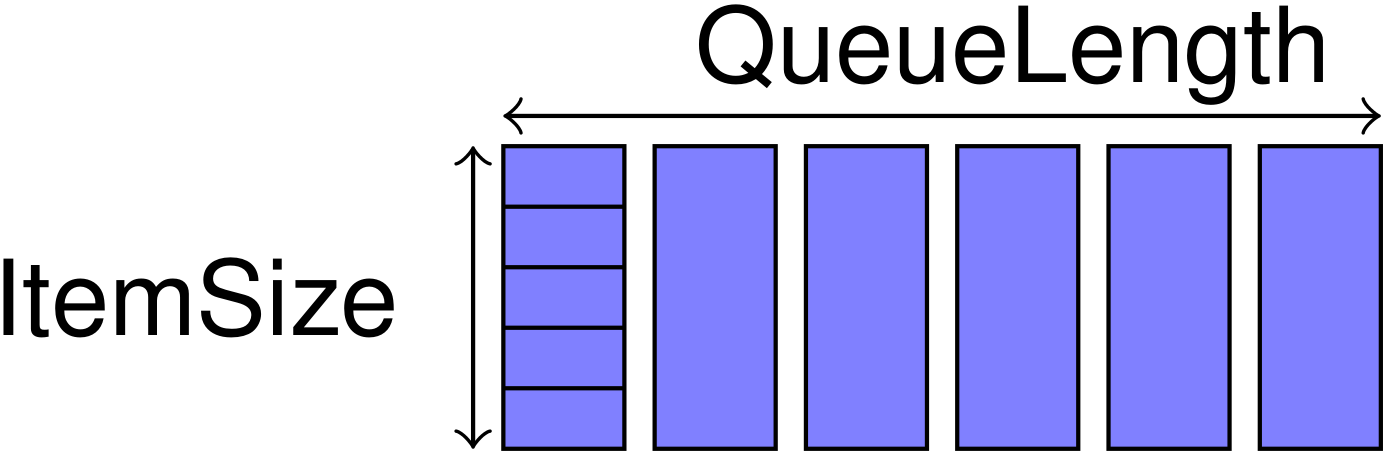
\includegraphics[scale=0.15]{pic/01_queue/queue_01.png} 
  %\caption{Prio Inheritance}
  \end{figure}
  
  \begin{figure}
  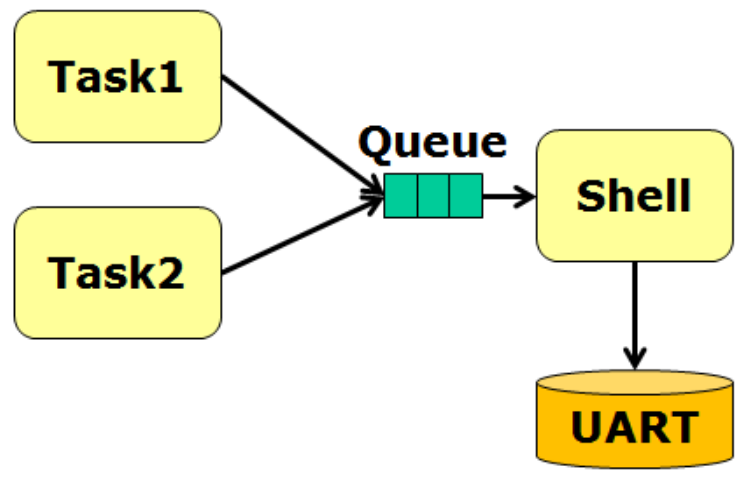
\includegraphics[scale=0.15]{pic/01_queue/queue_02.png} 
  %\caption{Prio Inheritance}
  \end{figure}
  
  
\end{frame}


\begin{frame}
  \frametitle{Add item}
%	\begin{lstlisting}
%	BaseType_t xQueueSendToBack (
%	  xQueueHandle xQueue ,
%	  const void ∗ pvItemToQueue ,
%	  portTickType xTicksToWait
%	  );
%	BaseType_t xQueueSendToFront (
%	  xQueueHandle xQueue ,
%	  const void ∗ pvItemToQueue ,
%	  portTickType xTicksToWait
%	);
%	\end{lstlisting}
\end{frame}


\section{Semaphore}
\begin{frame}
	%\frametitle{Semaphore}
  \tableofcontents[
	    currentsection, 
	    hideothersections, 
	    sectionstyle=show/shaded, 
	    subsectionstyle=hide
	]
\end{frame}


\begin{frame}
  \frametitle{Übersicht}
	\begin{itemize}
	  \item Primitive Lösung für Synchronisation.
	  \item Thread übergreifende Datenaustausch 
	  \item Nicht geschützt gegen Interrupts!!!
	\end{itemize}
\end{frame}



% ----------------------------------------------
%
% Prio Inheritage
%
% ----------------------------------------------
\begin{frame}
  \frametitle{Prioritäten Inversion - Vererbung}
  Problem: Priorität Inversion
	\begin{itemize}
	  \item Tiefere priorität blockiert höhere Priorität
	\end{itemize}
	Lösung:
  \begin{itemize}
	  \item Prioräten Vererbung: "Lower-prio task inherits the prio of any higher-prio task pending on resource"
	\end{itemize}
	\bigskip
	Death locks weiterhin möglich
\end{frame}


\begin{frame}
  \frametitle{Prio Inheritance}
  \begin{figure}
  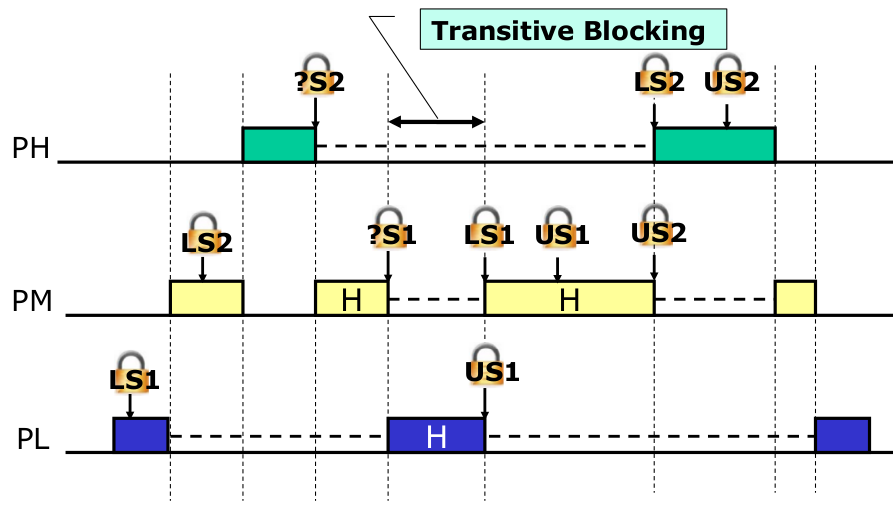
\includegraphics[scale=0.3]{pic/02_sem/sem_01.png} 
  %\caption{Prio Inheritance}
  \end{figure}
\end{frame}


% ----------------------------------------------
%
% Prio Ceiling
%
% ----------------------------------------------
\begin{frame}
  \frametitle{Prioritäten Inversion - "Ceiling"}
  Problem: Priorität Inversion
	\begin{itemize}
	  \item Tiefere priorität blockiert höhere Priorität
	  \item Death locks
	\end{itemize}
	Lösung:
  \begin{itemize}
	  \item Prioräten Vererbung: "Lower-prio task inherits the prio of any higher-prio task pending on resource"
	\end{itemize}
	\bigskip
	Deathlocks weiterhin möglich
\end{frame}

\begin{frame}
  \frametitle{Prio Ceiling}
  \begin{figure}
  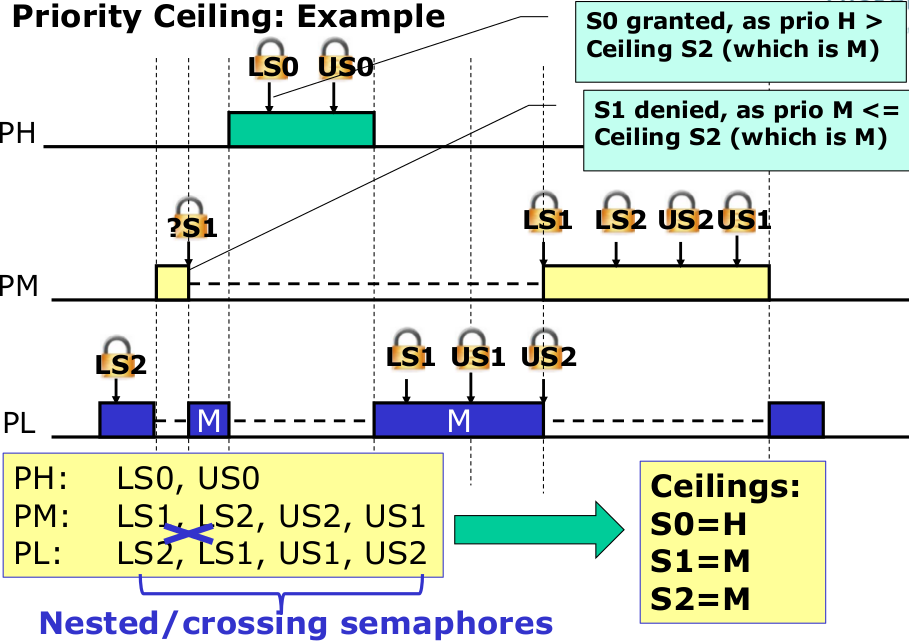
\includegraphics[scale=0.3]{pic/02_sem/sem_02.png} 
  %\caption{Prio Inheritance}
  \end{figure}
\end{frame}
\section{Mutex}
\begin{frame}
	%\frametitle{Mutex}
  \tableofcontents[
	    currentsection, 
	    hideothersections, 
	    sectionstyle=show/shaded, 
	    subsectionstyle=hide
	]
\end{frame}


\begin{frame}
  \frametitle{Mutex}
	\begin{itemize}
	\item Binärer Semaphore
	\item Ressourcen schützen, 1 Thread in kritischer Section
	\item Muss immer freigegeben werden!!!
	\item Priority Inheritance --> Deathlock möglich
	\item Nicht geschützt gegen Interrupts!!!
	\end{itemize}
\end{frame}







\end{document}